\documentclass[10pt]{standalone}
\usepackage[utf8]{inputenc}
\usepackage{pgf,tikz,pgfplots}
\pgfplotsset{compat=1.15}
\usepackage{mathrsfs}
\usetikzlibrary{arrows}
\pagestyle{empty}
\begin{document}

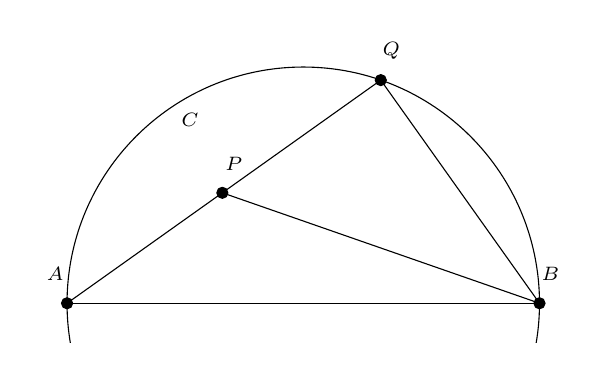
\begin{tikzpicture}[line cap=round,line join=round,>=triangle 45,x=1.0cm,y=1.0cm]

\clip(-0.5,-0.5) rectangle (6.5,3.5);
\draw  (3.,0.) circle (3.cm);
\draw  (0.,0.)-- (6.,0.);
\draw  (0.,0.)-- (3.9844047938229687,2.833892588278243);
\draw  (3.9844047938229687,2.833892588278243)-- (6.,0.);
\draw  (1.9722601452080204,1.4027624442994568)-- (6.,0.);
\begin{scriptsize}
\draw [fill=black] (0.,0.) circle (2.0pt);
\draw (-0.15,0.37) node {$A$};
\draw [fill=black] (6.,0.) circle (2.0pt);
\draw (6.14,0.37) node {$B$};
\draw (1.56,2.33) node {$C$};
\draw [fill=black] (3.9844047938229687,2.833892588278243) circle (2.0pt);
\draw (4.12,3.21) node {$Q$};
\draw [fill=black] (1.9722601452080204,1.4027624442994568) circle (2.0pt);
\draw (2.12,1.77) node {$P$};
\end{scriptsize}

\end{tikzpicture}
\end{document}